\section{Before starting}
\sectionframe	% section title is automatically capitalised

\begin{frame}
    \frametitle{Create a Virtual Network}
    \begin{center}
        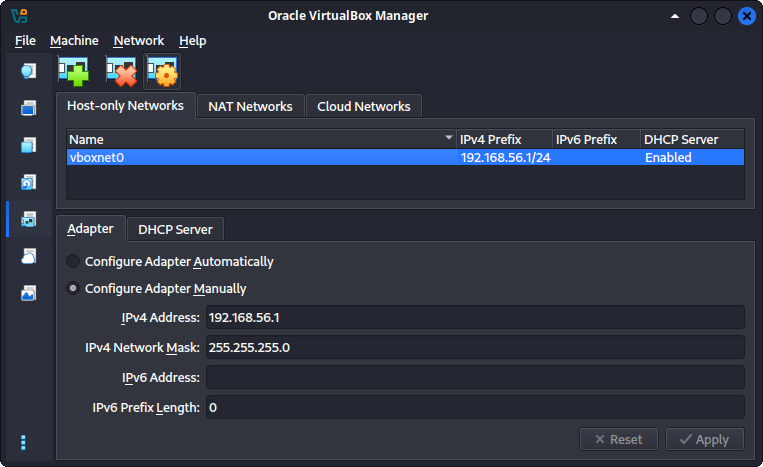
\includegraphics[width=0.48\textwidth]{images/net_setup_1.png}
        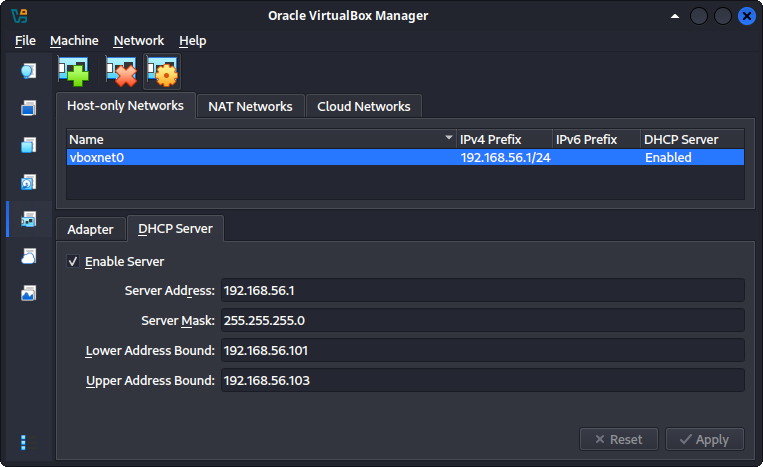
\includegraphics[width=0.48\textwidth]{images/net_setup_2.png}
    \end{center}
    \begin{enumerate}
        \item Go to Networks Settings and create a new Host-only Network
        \item Enable DHCP server and set the IP range enough to accommodate 3 VMs
        \item Save the configuration and remember the name of the network
    \end{enumerate}
\end{frame}

\begin{frame}
    \frametitle{Configure VM Network Settings}
    \begin{columns}[T,onlytextwidth]
        \begin{column}{0.4\textwidth}
            These are the 3 VMs:
            \begin{itemize}
                \item OPENVAS-FREE-24.10.9-VirtualBox
                \item Debian
                \item Windows XP
            \end{itemize}
            Configure the Network \underline{of all of them}
            by selecting the \textbf{Host-only Adapter} as network adapter 
            and choosing the network you created in the previous step.
        \end{column}
        \begin{column}{0.6\textwidth}
            \centering
            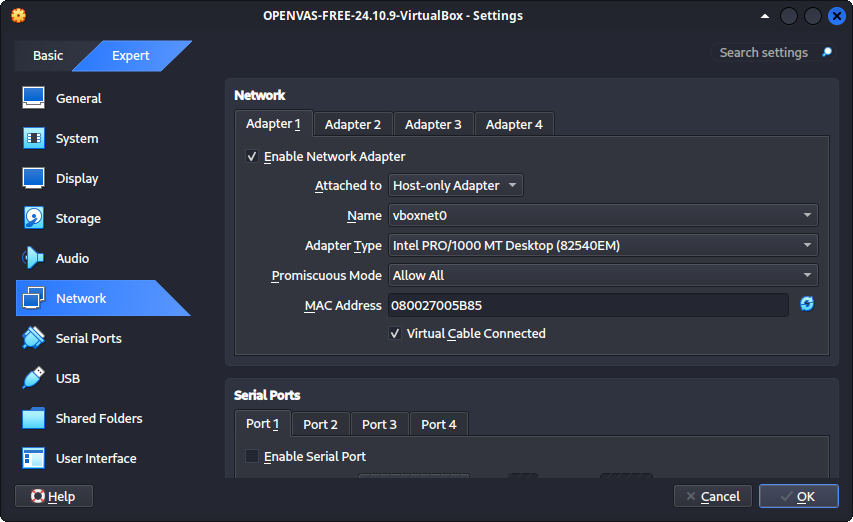
\includegraphics[width=\textwidth]{images/net_setup_3.png}
        \end{column}
    \end{columns}
\end{frame}

\begin{frame}[fragile]
    \frametitle{Start VMs without GUI}
    \begin{center}
        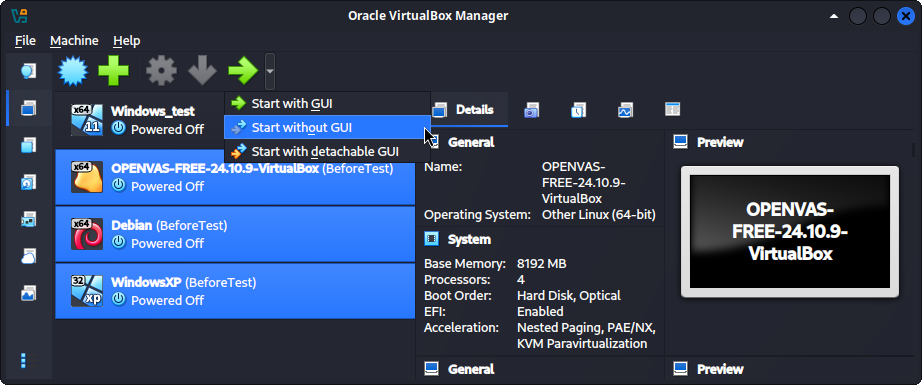
\includegraphics[width=0.8\textwidth]{images/vb-startup.png}
    \end{center}
    In order to save as much resources as possible, we will start the VMs without GUI.
    And since it will take a while to start, we will start them now and let them run in the background while we talk about the theory.
\end{frame}
